\chapter{Results}
\label{ch:results}

% SOURCE OF TRUTH: thesis-pack/00-start-here/RESULTS.md. Every number in this
% chapter comes from there. Where any other document disagrees, RESULTS wins.
% The exploratory Protocol v2 instruments (regret, loss attribution, handshake
% closure, coordination surface, commitment integrity) are reported here only
% where they are needed to read a confirmatory number. Their full treatment is
% Chapter~\ref{ch:critique}.
%
% RULES FOR THIS CHAPTER, from thesis-pack/README.md:
%  * Never write that the baseline "adapted", "recovered" or "replanned better".
%    Its S = 1.000 is the null policy's score.
%  * The agentic deficit is a COMMITMENT failure, not a handshake failure.
%  * Quote the CAPPED survival column for qwen3.5 and state the cap.
%  * Do not soften the deficit. Do not apologise for it either.

This chapter reports what the evaluation measured. It follows the design frozen
in Chapter~\ref{ch:eval} and changes nothing in it. The order is the order of
the gates: what was run, how the two systems did on the anticipated
disruptions, how they did on the novel ones, what the losses were made of, and
what the secondary measures add. Interpretation is held back for
Chapter~\ref{ch:discussion}. The criticism of the method itself is
Chapter~\ref{ch:critique}.

One result carries the chapter. The workflow baseline beats the
database-centric agentic system on resident survival in every disruption that
was tested. Both pre-registered hypotheses fail. Gate~1 fails in 26 of its 27
cells. That is the finding, and the rest of the chapter is the detail behind
it.

\section{Execution Summary}
\label{sec:res:summary}

The evaluation ran 310 scored runs. All 310 were eligible. None was censored,
none was left unscored, and no run carried an invalid model binding.
Table~\ref{tab:res:whatran} lists what was executed.

\begin{table}[htbp]
\centering
\caption{What was run.}
\label{tab:res:whatran}
\small
\begin{tabularx}{\textwidth}{l>{\raggedright\arraybackslash}X}
\toprule
Case & Augustinum nursing home, 100 residents, Hamburg storm surge. Feasibility ceiling 100 residents. \\
Systems & \texttt{agentic} (10 agents across 8 organizations, database-centric) against \texttt{baseline} (workflow). \\
Anticipated arm & \code{closed_loop} and \code{road_closure}. Both were visible during development. \\
Novel arm & Five disruptions supplied by the supervisor and held out: \code{medical_emergency_in_flight}, \code{unverified_persons_report}, \code{conflicting_evacuation_orders}, \code{bus1_suspension_capacity_reduction}, \code{sc1_partial_capacity_loss}. \\
Replicates & $k = 10$ per cell, replicates 1000 to 1009, paired baseline and agentic under common random numbers. \\
Scale & \code{SIM_TIME_SCALE} = 8.4, one value only. \\
Scored runs & 310. Zero censored, zero unscored, zero invalid model bindings. \\
Primary outcome & Recovery-Outcome Level 0 to 4, and survival $S$ = valid residents divided by the feasibility ceiling. \\
\bottomrule
\end{tabularx}
\end{table}

Three models completed the full novel arm at 50 runs each. These are glm-5.2,
deepseek-v4-pro and qwen3.5. Four further models hold partial series: kimi-k3
with 11 runs, gpt-oss with 4, kimi-k2.7-code with 3, and from the earlier
campaign minimax-m3 and nemotron-3-ultra on the anticipated arm only. Partial
series are reported on their own and are never pooled with the full arms. Section~\ref{sec:res:models} explains why.

An audit of all 218 novel-arm runs checked coverage, duplicates, model binding,
manifests and provenance. Coverage is 50 of 50 on each full arm. There are no
duplicate run identifiers, no duplicate cell identifiers and no duplicate log
checksums. All 218 manifests are present. There are zero model-binding errors,
zero undelivered world commands, and every scenario hash stayed stable for the
whole arm. The threshold file hash \texttt{d08c1e35} is identical across all
310 runs, so every run was scored against the same frozen thresholds.

Two things about the run set have to be said here, because they change how a
reader should treat some of the tables that follow.

\textbf{28 of 168 agentic novel runs did not quiesce.} They are marked
``stopped without quiescence: the final turn may be missing''. This is 17\% of
that set and it is spread across models. The outcome was decided in all of
them, so every run is scorable. A final message may be missing from the log.

\textbf{Two runs executed on a dirty working tree.} Runs \texttt{5f5b6b1e} and
\texttt{7e74e997} are the deepseek \code{unverified_persons_report}
replicates 1001 and 1002. They ran with uncommitted routing changes that were
committed later. The protocol does not admit this as a reason to exclude a run,
so both are kept and disclosed here.

\section{Anticipated Disruptions}
\label{sec:res:anticipated}

The anticipated arm is the precondition, not the result. It asks whether the
agentic system is at least as good as the baseline on disruptions that the
baseline was written for. That is hypothesis H1, and it is tested as
non-inferiority against a margin $\delta_{NI} = 0.05$.

\begin{table}[htbp]
\centering
\caption{Anticipated arm, mean survival $S$.}
\label{tab:res:anticipated}
\begin{tabular}{lcc}
\toprule
System and model & \code{closed_loop} & \code{road_closure} \\
\midrule
baseline & 1.000 & 1.000\textsuperscript{*} \\
agentic / glm-5.2 & \textbf{1.000} (pass) & 0.840 \\
agentic / qwen3.5 & 0.950\textsuperscript{\dag} & not run \\
agentic / deepseek-v4-pro & 0.790 & 0.700 \\
agentic / minimax-m3 & 0.340 & 0.150 \\
agentic / nemotron-3-ultra & 0.000 ($n=2$) & not run \\
\bottomrule
\end{tabular}
\end{table}

\textbf{H1 is rejected.} Non-inferiority holds in 1 of the 8 anticipated cells
and fails in the other 7. The one pass is glm-5.2 on \code{closed_loop},
where the risk difference is exactly 0.000. That cell is the undisrupted
scenario, and it is the only place in the whole evaluation where the agentic
system is demonstrably not worse than the baseline.

Two footnotes to Table~\ref{tab:res:anticipated} matter more than footnotes
usually do.

\textsuperscript{*} On \code{road_closure} the baseline's feasibility ceiling
fell to 60 for all 10 runs, because the shelters it heard from declared fewer
beds. Its $S$ of 1.000 is therefore measured against a reduced denominator. Its
completeness against the nominal 100 residents is \textbf{0.60}. Whenever the
baseline's \code{road_closure} result is compared with anything else, the
nominal figure is the one to quote.

\textsuperscript{\dag} The qwen3.5 \code{closed_loop} cell was added under
Amendment~13 to complete that model's level ladder, which
Section~\ref{sec:res:models} explains. Its risk difference is $-0.05$
[$-0.15$, $0.00$] and Gate~1 reads \texttt{fail}. Its levels are six runs at
level 4, three at level 3 and one at level 2. qwen3.5 has no
\code{road_closure} cells, because it was never a campaign model.

\section{Novel Disruptions}
\label{sec:res:novel}

The novel arm is the primary test. Five disruptions were supplied by the
supervisor, held out from development, and revealed on evaluation day. The
baseline has no written branch for any of them. Hypothesis H2 predicted that
the agentic system would win here.

% TODO(figure): mean S per disruption, baseline against the three full models.
% Source: thesis-pack/00-start-here/RESULTS.md sec. 2. Grouped bar chart.

\subsection{Survival}
\label{sec:res:novel:survival}

\begin{table}[htbp]
\centering
\caption{Novel arm, mean survival $S$ over all 50 runs per model against the
50 paired baseline runs.}
\label{tab:res:novelmeans}
\begin{tabular}{lccccc}
\toprule
System and model & $n$ & mean $S$ & capped $S$ & median level & level-4 runs \\
\midrule
\textbf{baseline} & 50 & \textbf{1.000} & 1.000 & 4 & 50 \\
agentic / qwen3.5 & 50 & 0.900 & \textbf{0.894} & 4 & 30 \\
agentic / glm-5.2 & 50 & 0.840 & 0.840 & 4 & 31 \\
agentic / deepseek-v4-pro & 50 & 0.727 & 0.727 & 2 & 15 \\
\bottomrule
\end{tabular}
\end{table}

The baseline scored a perfect 1.000 on all 50 novel runs. The best agentic
configuration reached 0.894.

The capped column is the one to read. Three qwen3.5 runs scored above the
feasibility ceiling and are capped at 1.0. Section~\ref{sec:res:integrity}
explains the defect behind them. Capping moves qwen3.5's novel mean from 0.900
to 0.894 and changes no conclusion anywhere in this chapter.

Per disruption the picture is the same in every cell.

\begin{table}[htbp]
\centering
\caption{Novel arm, mean survival $S$ per disruption.}
\label{tab:res:noveldisruption}
\small
\begin{tabular}{lcccc}
\toprule
Disruption & baseline & qwen3.5 & glm-5.2 & deepseek \\
\midrule
\code{conflicting_evacuation_orders} & 1.000 & \textbf{0.980} & 0.850 & 0.650 \\
\code{medical_emergency_in_flight} & 1.000 & \textbf{0.920} & 0.850 & 0.800 \\
\code{bus1_suspension_capacity_reduction} & 1.000 & \textbf{0.920} & 0.850 & 0.755 \\
\code{unverified_persons_report} & 1.000 & \textbf{0.900} & 0.840 & 0.690 \\
\code{sc1_partial_capacity_loss} & 1.000 & 0.780 & \textbf{0.810} & 0.740 \\
\bottomrule
\end{tabular}
\end{table}

\subsection{Gate 1: Survival}
\label{sec:res:novel:gate1}

Gate~1 spans both arms and reads a different hypothesis on each, because the
two arms ask different questions of the same quantity. On the anticipated arm
it is a non-inferiority test and carries H1. On the novel arm it is a
superiority test and carries H2. Table~\ref{tab:res:gate1} gives the count.

\begin{table}[htbp]
\centering
\caption{Gate~1 across both arms.}
\label{tab:res:gate1}
\small
\begin{tabular}{llccc}
\toprule
Arm & Test & Hypothesis & Cells & Pass \\
\midrule
Anticipated & non-inferiority against $\delta_{NI} = 0.05$ & H1 & 8 & 1 \\
Novel & superiority, paired CI excluding zero & H2 & 19 & 0 \\
\midrule
 & & & \textbf{27} & \textbf{1} \\
\bottomrule
\end{tabular}
\end{table}

\textbf{Gate~1 fails in 26 of 27 cells.} The single pass anywhere in the
evaluation is glm-5.2 on \code{closed_loop}. That pass is a non-inferiority
result on the anticipated arm. It is not a superiority result, and Gate~1 as a
whole is not a superiority test. The novel-arm failures also belong to H2, not
to H1. H2 is the hypothesis that predicted an agentic win where the baseline
had no written branch.

The risk difference is $RD = S_{\text{agentic}} - S_{\text{baseline}}$,
computed paired, with a positive value favouring the agentic system.
Table~\ref{tab:res:rd} gives all 15 novel cells with bootstrap confidence
intervals.

\begin{table}[htbp]
\centering
\caption{Novel-arm risk differences with bootstrap confidence intervals.
Positive favours the agentic system. Every cell is negative.}
\label{tab:res:rd}
\scriptsize
\setlength{\tabcolsep}{4pt}
\begin{tabular}{lccc}
\toprule
Disruption & qwen3.5 & glm-5.2 & deepseek \\
\midrule
\code{conflicting_evacuation_orders} & $-0.02$ [$-0.05$, $0.00$] & $-0.15$ [$-0.30$, $0.00$] & $-0.35$ [$-0.55$, $-0.17$] \\
\code{medical_emergency_in_flight} & $-0.08$ [$-0.21$, $0.02$] & $-0.15$ [$-0.30$, $0.00$] & $-0.20$ [$-0.42$, $-0.04$] \\
\code{bus1_suspension_capacity_reduction} & $-0.08$ [$-0.18$, $-0.01$] & $-0.15$ [$-0.30$, $0.00$] & $-0.245$ [$-0.45$, $-0.08$] \\
\code{unverified_persons_report} & $-0.10$ [$-0.23$, $0.00$] & $-0.16$ [$-0.31$, $-0.03$] & $-0.31$ [$-0.44$, $-0.17$] \\
\code{sc1_partial_capacity_loss} & $-0.22$ [$-0.44$, $-0.03$] & $-0.19$ [$-0.42$, $0.00$] & $-0.26$ [$-0.52$, $-0.03$] \\
\bottomrule
\end{tabular}
\end{table}

\begin{figure}[htbp]
\centering
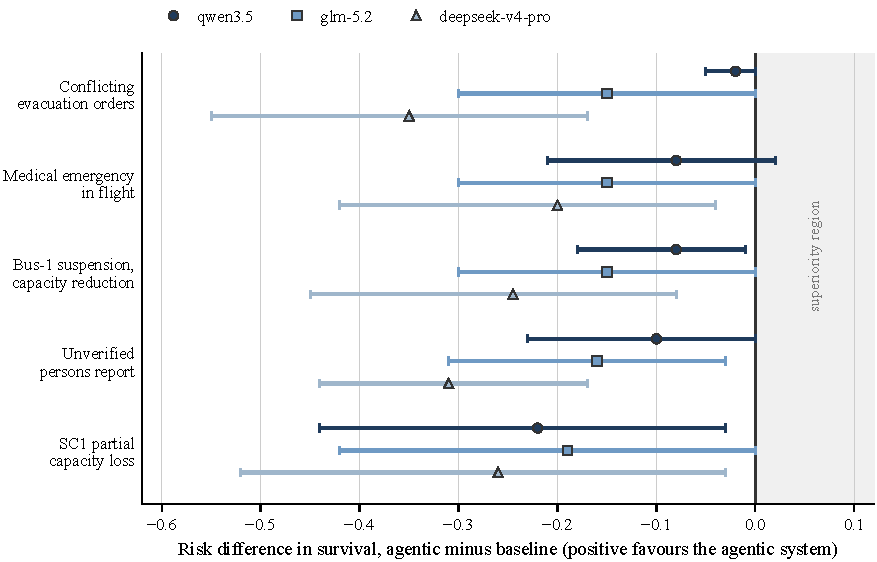
\includegraphics[width=\textwidth]{pics/results-forest-rd.pdf}
\caption[Novel-arm risk differences]{The 15 novel-arm risk differences with
their bootstrap confidence intervals. A superiority result would need the whole
interval to sit inside the shaded region. None does, and no point estimate is
positive. Table~\ref{tab:res:rd} gives the same values exactly. Drawn from
\texttt{data/novel\_risk\_differences.csv}.}
\label{fig:res:forest}
\end{figure}

Superiority needs the paired interval to exclude zero on the positive side. No
cell comes close. Every point estimate is negative.
Figure~\ref{fig:res:forest} shows why the verdict does not depend on reading
any single row. All 15 intervals lie to the left of zero. Eight stay strictly
below it, six reach zero and stop there, and exactly one reaches past it:
qwen3.5 on
\code{medical_emergency_in_flight}, whose upper bound is 0.02. The three models
also separate cleanly in the figure, which is the capability ordering that
Section~\ref{sec:res:models} returns to.

\subsection{The H2 Minimum Effect}
\label{sec:res:novel:delta}

H2 also set a minimum effect. It required a median shift of one whole recovery
level, $\delta_m = +1.0$, together with first-order stochastic dominance of the
agentic system over the baseline. Table~\ref{tab:res:levelshift} gives the
median paired level shift in each cell.

\begin{table}[htbp]
\centering
\caption{Median paired level shift, agentic minus baseline. The registered
minimum effect was $+1.0$.}
\label{tab:res:levelshift}
\small
\begin{tabular}{lccc}
\toprule
Disruption & qwen3.5 & glm-5.2 & deepseek \\
\midrule
\code{conflicting_evacuation_orders} & 0.0 & 0.0 & $-2.0$ \\
\code{medical_emergency_in_flight} & 0.0 & 0.0 & $-2.0$ \\
\code{unverified_persons_report} & 0.0 & $-0.5$ & $-2.0$ \\
\code{bus1_suspension_capacity_reduction} & $-0.5$ & $-0.5$ & $-2.0$ \\
\code{sc1_partial_capacity_loss} & $-1.0$ & 0.0 & 0.0 \\
\bottomrule
\end{tabular}
\end{table}

No cell is positive. Every novel row reads \code{below_delta_m} with
dominance assigned to the baseline, so neither of the two conditions holds
anywhere. The best the agentic system manages is parity of median level on four
of the five disruptions, and it reaches that parity while still losing
residents. That is exactly why Gate~1 fails where the median level does not.

\subsection{The Registered H2 Primary}
\label{sec:res:novel:prereg}

The pre-registration named a different primary test for H2. It registered an
exact Clopper-Pearson interval on $P(\text{level}_{\text{agentic}} \geq
\text{level}_{\text{baseline}})$ over the $k$ agentic runs against the
control's constant level, aggregated across scenarios by a sign test with
Holm-Bonferroni correction.

\textbf{That test was not implemented when the results above were first
written.} It was coded afterwards, once the result was already known. This is a
deviation from the pre-registration's timing and is reported as one. Under the
pre-registration's own rules the analysis is therefore exploratory.
Chapter~\ref{ch:critique} treats it properly. The numbers are given here
because they belong beside the verdict they check.

The control scored level 4 on all 50 novel runs, so the success event is that
the agentic run also reached level 4.

\begin{table}[htbp]
\centering
\caption{Registered H2 primary: successes out of 10 with exact
Clopper-Pearson intervals.}
\label{tab:res:cp}
\footnotesize
\begin{tabular}{lccc}
\toprule
Disruption & qwen3.5 & glm-5.2 & deepseek \\
\midrule
\code{conflicting_evacuation_orders} & 7/10 [0.35, 0.93] & 7/10 [0.35, 0.93] & 1/10 [0.00, 0.44] \\
\code{medical_emergency_in_flight} & 7/10 [0.35, 0.93] & 7/10 [0.35, 0.93] & 4/10 [0.12, 0.74] \\
\code{sc1_partial_capacity_loss} & 5/10 [0.19, 0.81] & 7/10 [0.35, 0.93] & 6/10 [0.26, 0.88] \\
\code{unverified_persons_report} & 6/10 [0.26, 0.88] & 5/10 [0.19, 0.81] & 2/10 [0.03, 0.56] \\
\code{bus1_suspension_capacity_reduction} & 5/10 [0.19, 0.81] & 5/10 [0.19, 0.81] & 2/10 [0.03, 0.56] \\
\bottomrule
\end{tabular}
\end{table}

The registered test agrees with the risk-difference verdict. Not one cell puts
the agentic system above chance. No interval has a lower bound above 0.5. One
cell sits below chance before correction, deepseek on
\code{conflicting_evacuation_orders} at 1 of 10 with $p = 0.021$, and it
does not survive the Holm correction, where $p = 0.107$.

The aggregation across scenarios is reported in Table~\ref{tab:res:signtest},
with one observation per scenario, because the pre-registration forbids pooling
runs across scenarios.

\begin{table}[htbp]
\centering
\caption{Registered scenario-level sign test. The last column is the smallest
$p$ the design could have produced for that model.}
\label{tab:res:signtest}
\small
\begin{tabular}{lcccccc}
\toprule
Model & scenarios & favour agentic & favour baseline & ties & $p$ & floor on $p$ \\
\midrule
qwen3.5 & 5 & 3 & 0 & 2 & 0.250 & \textbf{0.250} \\
glm-5.2 & 5 & 3 & 0 & 2 & 0.250 & \textbf{0.250} \\
deepseek-v4-pro & 5 & 1 & 4 & 0 & 0.375 & 0.0625 \\
\bottomrule
\end{tabular}
\end{table}

There is a second finding in that table, and it is about the design rather than
the systems. \textbf{At $k = 10$ this test can hardly conclude anything.} Every
Clopper-Pearson interval is about 0.6 wide, so even a cell at 7 of 10 cannot
separate from chance. The sign test is worse. A two-sided exact sign test on
five scenarios cannot return a $p$ below 0.0625 however the data fall, and ties
push the floor higher. qwen3.5 and glm-5.2 each tie two scenarios, which leaves
three untied observations and a floor of 0.250. Both models are therefore
already sitting at the smallest $p$ their data could have produced. The
registered aggregation cannot reach conventional significance in this design at
all.

This is why the risk difference carries the argument. It is continuous, it is
paired, and it is far more efficient with the replicates available. The
weakness of the registered plan is a limitation of the analysis plan, not a
result, and Chapter~\ref{ch:critique} takes it up as a methods finding.

One more warning about Table~\ref{tab:res:signtest}. The sign test's direction
is mildly favourable to qwen3.5 and glm-5.2, with three scenarios above chance,
none below and two tied, while both models still lose residents in every cell.
That is not a win. The sign test counts which side of 0.5 a cell falls on and
is blind to how far, which is precisely the information the risk difference
keeps.

\subsection{What the Novel Arm Does Not Show}
\label{sec:res:novel:boundary}

The novel arm answers whether the agentic system won on these scenarios. It
does not answer whether an agentic system can ever win, because no scenario in
this thesis ever \emph{required} adaptation. Chapter~\ref{ch:critique} shows
that a controller which ignores every disruption scores the same level as the
baseline on all five novel scenarios. The baseline's $S$ of 1.000 is the null
policy's score.

Two consequences follow, and both hold for every table in this chapter. First,
the baseline's result must never be described as recovery, adaptation or better
replanning. It did not adapt, because nothing it did changed an order or a
kilometre. Second, that withdrawal cuts one way only. It does not turn into an
agentic win. Against the same null policy the agentic regret is negative in all
15 novel cells, and 68 of 150 runs came out worse than doing nothing at all.

\section{What the Losses Were Made Of}
\label{sec:res:loss}

The survival tables say how much was lost. This section says what the loss was
made of, because the shape of the loss is what Chapter~\ref{ch:discussion}
builds on.

\subsection{Residents Never Moved}
\label{sec:res:loss:nevermoved}

\begin{table}[htbp]
\centering
\caption{Residents never moved, per 100. Lower is better.}
\label{tab:res:nevermoved}
\small
\begin{tabular}{lcccc}
\toprule
Disruption & baseline & qwen3.5 & glm-5.2 & deepseek \\
\midrule
\code{medical_emergency_in_flight} & 0.0 & \textbf{5.0} & 10.0 & 13.0 \\
\code{conflicting_evacuation_orders} & 0.0 & \textbf{2.0} & 15.0 & 19.0 \\
\code{bus1_suspension_capacity_reduction} & 0.0 & \textbf{2.0} & 15.0 & 22.5 \\
\code{unverified_persons_report} & 0.0 & \textbf{4.0} & 10.0 & 21.0 \\
\code{sc1_partial_capacity_loss} & 0.0 & \textbf{2.5} & 14.0 & 16.0 \\
\bottomrule
\end{tabular}
\end{table}

qwen3.5 strands far fewer residents than the other two models. It does so on
every disruption, by a factor of two to eight. Its survival deficit comes
mostly from residents arriving late or being invalidated by shelter overload,
not from residents left behind. That is a materially different failure from
deepseek's, and Section~\ref{sec:res:models} returns to it.

These figures were corrected after the first write-up. The column was computed
as the ceiling minus sheltered residents with no floor at zero, and the
over-delivery runs of Section~\ref{sec:res:integrity} drove two cells negative.
It is now floored at zero. Five cells changed. No confirmatory number moved.

\subsection{Late Arrivals and Shelter Overload}
\label{sec:res:loss:totals}

The two recorded loss mechanisms are residents who missed their deadline and
residents invalidated because a shelter was filled past what it declared.
Table~\ref{tab:res:lossmech} gives the totals. The scope has to be stated with
them, because the figures differ by nearly a factor of two depending on which
runs are counted.

\begin{table}[htbp]
\centering
\caption{Loss mechanism totals by scope.}
\label{tab:res:lossmech}
\small
\begin{tabular}{lccc}
\toprule
Scope & late arrivals & in runs & shelter-overload invalidations \\
\midrule
All agentic runs, both arms, all 7 models & 1\,675 & 41 & 215 \\
Agentic novel arm only & 1\,035 & 28 & 215 \\
Agentic novel arm, 3 full models only & 985 & 26 & 215 \\
\textbf{baseline, all runs} & \textbf{0} & \textbf{0} & \textbf{0} \\
\bottomrule
\end{tabular}
\end{table}

The figure of 1\,675 includes minimax-m3 and nemotron-3-ultra, and neither
model is part of the headline result. A novel-arm claim should quote the
novel-arm figure. The baseline recorded no late arrival and no overload in any
run.

\subsection{The Loss Is Not a Message-Layer Failure}
\label{sec:res:loss:handshakes}

An early reading of these results attributed the deficit to unanswered
handshakes. Measurement does not support that reading. Over 1\,932 addressed
requests in the agentic novel arm, handshake closure is \textbf{0.938}. The
three highest-volume handshakes close at 0.947, 0.970 and 0.997. The one weak
handshake is \code{abort_request} at 0.548, and it sits on a small
denominator of 31 requests.

The dominant mechanism is residents who were never dispatched at all. Across
the 150 agentic novel runs from the three full models, the correlation of
never-dispatched residents with $S$ is $r = -0.745$, against $-0.579$ for late
arrivals and $+0.061$ for shelter overload. The failure is in what the agents
committed to move, not in whether their messages arrived.

These are exploratory Protocol~v2 instruments, written after the data were
seen. They change no confirmatory number. Chapter~\ref{ch:critique} reports
them in full, together with the alternative explanations that were ruled out.

\subsection{The Loss Is Quantised}
\label{sec:res:loss:quantised}

Figure~\ref{fig:res:delivery} gives the distribution of residents delivered
across the same 150 runs. The shape is the argument.

\begin{figure}[htbp]
\centering
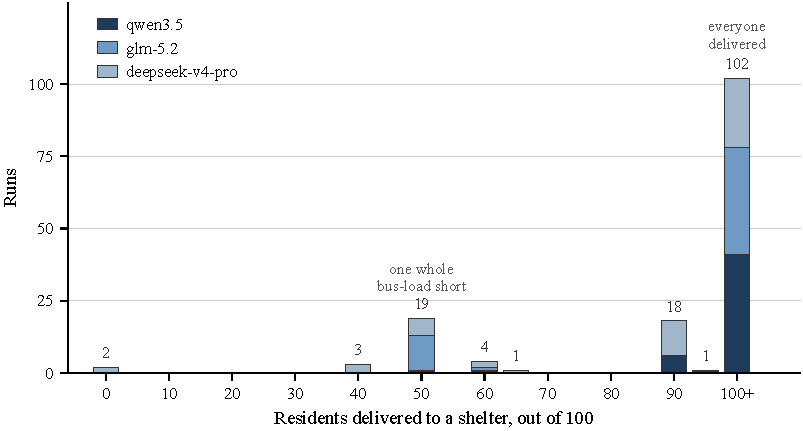
\includegraphics[width=\textwidth]{pics/results-delivery-histogram.pdf}
\caption[Residents delivered per run]{Residents delivered to a shelter, over
the 150 agentic novel runs from the three full models. The distribution
clusters on a few discrete values instead of spreading smoothly. The six runs
that report more arrivals than the ceiling admits
(Section~\ref{sec:res:integrity}) are folded into the \mbox{100+} column, the
same way the survival tables cap them. Drawn from
\texttt{data/delivery\_distribution.csv}.}
\label{fig:res:delivery}
\end{figure}

Of the 150 runs, 102 delivered everyone. Nineteen delivered exactly 50, which
is one whole bus-load short. Eighteen delivered exactly 90, and two delivered
nobody at all. Nothing lands between 65 and 90, and nothing lands between 10
and 40.

A system degrading under load does not produce that picture. It produces a
spread. A system that loses discrete committed legs does produce it. Together
with the 0.938 handshake closure, this is what moves the diagnosis from
comprehension to commitment: the agents understood the disruption and were
heard, and then failed to carry a plan they had already committed to through to
the end.

The figure also separates the models. The spike at 50 is mostly glm-5.2, with
12 of its 19 runs. The spike at 90 is mostly deepseek-v4-pro, with 12 of 18.
qwen3.5 holds 41 of the 102 full deliveries. This is descriptive and
exploratory, and Chapter~\ref{ch:critique} carries the causal argument and its
limits.

\section{Decision Quality}
\label{sec:res:quality}

Decision quality was measured by a held-out rubric applied to the novel arm.
The rubric is a secondary, structural measure. It is never tabulated beside a
recovery level, and it does not enter any gate. Each cell counts \texttt{yes}
judgements out of 10. A cell short of 10 had the remainder judged \texttt{no}
or \texttt{unanswerable}.

Table~\ref{tab:res:rubric} gives all five novel disruptions and all sixteen
criteria.

% TODO(figure): the 16-criteria split drawn as three bands (parity on 5,
% baseline wins 5, scenario-indicting 3). Source: RESULTS.md sec. 4.

\begin{table}[htbp]
\centering
\caption{Held-out decision rubric, \texttt{yes} judgements out of 10.}
\label{tab:res:rubric}
\footnotesize
\begin{tabular}{lcccc}
\toprule
Criterion & baseline & qwen3.5 & glm-5.2 & deepseek \\
\midrule
\multicolumn{5}{l}{\emph{Disruption:} \code{bus1_suspension_capacity_reduction}} \\
\quad \code{reserve_committed} & 10 & \textbf{10} & \textbf{10} & 9 \\
\quad \code{whole_population_planned} & 10 & \textbf{10} & \textbf{10} & 6 \\
\quad \code{bus_load_within_cap} & 0 & 0 & 3 & 2 \\
\midrule
\multicolumn{5}{l}{\emph{Disruption:} \code{conflicting_evacuation_orders}} \\
\quad \code{authority_informed} & 10 & \textbf{10} & 9 & \textbf{10} \\
\quad \code{full_evacuation_kept} & 10 & 9 & \textbf{10} & 5 \\
\quad \code{facility_answered_in_time} & \textbf{10} & 0 & 0 & 0 \\
\midrule
\multicolumn{5}{l}{\emph{Disruption:} \code{medical_emergency_in_flight}} \\
\quad \code{authority_informed} & 10 & \textbf{10} & \textbf{10} & \textbf{10} \\
\quad \code{in_flight_leg_lands_where_ordered} & 10 & 8 & 6 & 6 \\
\quad \code{medic_sent_to_the_bus_destination} & 0 & 1 & 1 & 0 \\
\midrule
\multicolumn{5}{l}{\emph{Disruption:} \code{unverified_persons_report}} \\
\quad \code{verification_requested} & 10 & 9 & \textbf{10} & \textbf{10} \\
\quad \code{stood_down_after_retraction} & 10 & \textbf{10} & \textbf{10} & 8 \\
\quad \code{reserve_committed_in_time} & 10 & 9 & \textbf{10} & 9 \\
\quad \code{facility_runs_untouched} & \textbf{10} & 7 & 8 & 5 \\
\midrule
\multicolumn{5}{l}{\emph{Disruption:} \code{sc1_partial_capacity_loss}} \\
\quad \code{no_order_raises_shelter_above_beds} & \textbf{10} & 5 & 9 & 8 \\
\quad \code{shelter_set_down_within_beds} & 0 & 2 & 2 & 0 \\
\quad \code{everyone_bedded_at_the_reduced_capacity} & 0 & 0 & 0 & 0 \\
\bottomrule
\end{tabular}
\end{table}

Read across all sixteen criteria, the rubric splits three ways.

\begin{sloppypar}
\textbf{Parity on five criteria.} These are \code{authority_informed} on both
disruptions, \code{reserve_committed}, \code{whole_population_planned} and
\code{stood_down_after_retraction}. qwen3.5 and glm-5.2 match the baseline's 10
out of 10 on all of them. This is the evidence that the agents reason about the
disruption correctly.

\textbf{The baseline wins on five criteria.} The clearest is
\code{facility_answered_in_time}, where the baseline scores 10 and no agentic
model ever answered the facility in time. The others are
\code{no_order_raises_shelter_above_beds} at 10 against 5, 9 and 8,
\code{facility_runs_untouched} at 10 against 7, 8 and 5,
\code{in_flight_leg_lands_where_ordered} at 10 against 8, 6 and 6, and
\code{full_evacuation_kept} at 10 against 9, 10 and 5.
\end{sloppypar}

\textbf{Three criteria indict the scenario rather than either architecture.}
\code{bus_load_within_cap},
\code{medic_sent_to_the_bus_destination} and
\code{everyone_bedded_at_the_reduced_capacity} score 0 for the baseline
too. They cannot be reported as agentic failures. On
\code{shelter_set_down_within_beds} the agentic side actually beats the
baseline, at 2 and 2 against 0.

\textbf{Decision quality is split, not at parity.} Over the sixteen criteria
the agentic models match the baseline on five and fall short on five. Parity
holds on the criteria about deciding, and fails on the criteria about closing
the loop. This chapter does not round that to decision-quality parity, and
neither does any later chapter.

\section{Response Time and Cost}
\label{sec:res:responsetime}

The baseline's model latency is 0.0 seconds by construction, because it runs no
model at all. Agentic wall-clock latency per run ranges from 763 seconds for
deepseek on \code{closed_loop} to 3\,810 seconds for kimi-k3 on
\code{medical_emergency_in_flight}. Within the three full novel arms the
per-cell means sit between 815 seconds, for deepseek on
\code{unverified_persons_report}, and 2\,528 seconds, for glm-5.2 on
\code{bus1_suspension_capacity_reduction}.

Bus kilometres are comparable only within a system, not between the two,
because the systems compose the total differently. The baseline drove 60.63
bus-km on every novel scenario, and the same 60.63 undisrupted. That single
fact is one of the reasons Chapter~\ref{ch:critique} exists.

The coordination surface is the cost that the original protocol never printed.
Table~\ref{tab:res:surface} gives it for the 150 agentic novel runs and their
50 paired control runs. These are exploratory Protocol~v2 figures.

\begin{table}[htbp]
\centering
\caption{Coordination surface on the novel arm. Exploratory.}
\label{tab:res:surface}
\footnotesize
\begin{tabular}{lcccccc}
\toprule
System and model & nodes & messages & decisions & msgs / resident & tokens & budget fraction \\
\midrule
baseline & 2 & 13.2 & 13.2 & \textbf{0.13} & 0 & 0.00 \\
agentic / deepseek-v4-pro & 11 & 91.9 & 152.6 & 1.26 & 725\,457 & 1.80 \\
agentic / qwen3.5 & 11 & 106.6 & 170.3 & 1.18 & 894\,243 & 2.28 \\
agentic / glm-5.2 & 11 & 111.8 & 174.9 & 1.33 & 829\,906 & 2.70 \\
\bottomrule
\end{tabular}
\end{table}

The control coordinates a hundred-resident evacuation on 13 messages into one
node. The agentic system spends seven to eight and a half times as many
messages across eleven nodes, which is nine to ten times as many per resident
delivered. It also spends roughly 800\,000 tokens and 1.8 to 2.7 times the
wall-clock that the compressed clock allows. 140 of the 150 runs finished over
budget.

On these scenarios that surface bought nothing. Whether it buys anything on a
scenario that actually requires adaptation is an open question, and this design
cannot answer it.

\section{Process Diagnostics}
\label{sec:res:diagnostics}

Process diagnostics explain the outcome distribution. They do not score it.
Supersede count in particular rewards churn, and the protocol demotes it on
purpose.

The diagnostic that turned out to matter is the number of plan revisions.
Table~\ref{tab:res:commitment} bands the 150 agentic novel runs by it.

% TODO(figure): plan revisions against full-delivery rate, 90 % down to 32 %.
% Source: EVALUATION_PROTOCOL_V2.md sec. 11.4.

\begin{table}[htbp]
\centering
\caption{Plan revisions against delivery, 150 agentic novel runs.
Exploratory.}
\label{tab:res:commitment}
\small
\begin{tabular}{lcccc}
\toprule
Plan revisions & runs & mean $S$ & mean aborts & full delivery \\
\midrule
2 (the minimum) & 61 & 0.923 & 0.08 & \textbf{90\%} \\
3 & 22 & 0.827 & 0.55 & 77\% \\
4 & 15 & 0.853 & 0.67 & 67\% \\
5 & 11 & 0.782 & 1.27 & 64\% \\
6 or more & 41 & 0.670 & 1.63 & \textbf{32\%} \\
\bottomrule
\end{tabular}
\end{table}

The full-delivery rate falls monotonically across the bands, from 90\% at the
minimum revision count to 32\% at six or more. The correlation of plan
revisions with $S$ is $r = -0.408$, which is the strongest non-definitional
predictor in the data. Aborts correlate at $r = -0.306$. The number of missions
dispatched correlates at only $r = -0.070$, so it is not how many missions were
ordered but how many times the plan was rewritten.

The causal direction is not established, and this chapter does not claim it. Of
108 aborts, 52.8\% are explicit post-failure stand-downs and only 13.0\% are
clearly revision-initiated. A run that is going badly plausibly re-plans because
it is going badly. Observational data cannot separate the two directions.
Chapter~\ref{ch:critique} names the experiment that would.

\section{Model Sweep and Capability Threshold}
\label{sec:res:models}

The gap narrows with model capability. The mean novel-arm risk difference is
$-0.27$ for deepseek-v4-pro, $-0.16$ for glm-5.2 and $-0.10$ for qwen3.5. The
ordering is consistent across all five novel disruptions. On four of the five,
qwen3.5 matches the baseline's median level while still losing residents, so it
reaches the same recovery category without the same survival.

The weaker models fail badly rather than narrowly. minimax-m3 scored 0.340 on
\code{closed_loop} and 0.150 on \code{road_closure}. nemotron-3-ultra
scored 0.000 on the two runs it completed. Neither model is part of the
headline result.

No capability threshold is observable inside the final model set, and the
design does not support extrapolating past qwen3.5.

\textbf{Hypothesis H3 cannot be resolved, because it presupposes H2.} H3
predicted that the agentic advantage on novel disruptions would be
model-robust, with a capability threshold below which that advantage
disappears. There is no advantage here to be robust or fragile. The threshold
H3 asks about is therefore undefined rather than unobserved, and no verdict on
H3 is reported. What the model sweep does establish is the ordering above: the
size of the deficit tracks model capability, consistently, across every novel
disruption. That is a descriptive finding and not the registered hypothesis.

\subsection{Why Levels Are Comparable for Three Arms Only}
\label{sec:res:models:levelcap}

A promotion to level 4 requires a resource-efficiency judgement against the
model's own no-disruption reference. That reference needs three qualifying
control runs. A model with no \code{agentic_closed_loop} runs is capped at
level 3 regardless of how well it performed.

qwen3.5 was originally novel-arm-only and was capped by this rule. It held the
best agentic survival with zero level-4 runs, which made every level-based
comparison involving it an artifact. Amendment~13 ran its ten anticipated
\code{closed_loop} cells to supply the reference. After re-scoring it has 30
level-4 runs and a median level of 4, against glm-5.2's 31 and 4. Levels are
now comparable across the three full arms.

Three series remain capped and are comparable on $S$ only. These are kimi-k3
with 11 runs at $S = 0.773$, kimi-k2.7-code with 3 runs at 0.667 and gpt-oss
with 4 runs at 0.375. They must never be ranked by level against the full arms.

Re-scoring changed no survival figure. $S$, $RD$ and Gate~1 are computed per
run and never consult the clean-run reference. The Gate~1 verdicts before and
after re-scoring are identical.

\subsection{The Third Model Slot Changed Four Times}
\label{sec:res:models:churn}

The novel arm's third model slot was held in turn by kimi-k3 with 11 runs,
gpt-oss with 4, kimi-k2.7-code with 3 and finally qwen3.5 with 50. Each swap
was made after seeing data. Under the pre-registration the novel arm's model
set, and any analysis using it, is therefore exploratory. The four short series
are reported separately and never pooled. glm-5.2 and deepseek-v4-pro were
fixed before the novel arm ran and are unaffected.

\section{Sensitivity Analysis}
\label{sec:res:sensitivity}

The protocol makes the cut-point sensitivity analysis a precondition on the
headline. Each cell's median level was re-read with the level 1 to 2 cut moved
to 0.40, 0.50 and 0.60. A cell is stable when it reads the same at all three
cuts.

\textbf{The result supports the headline.} Every cell in the three full novel
arms reads the same median at all three cuts, with one exception:
\code{unverified_persons_report} for deepseek moves from 2.0 to 1.5 at the
0.60 cut. The only other unstable cells are minimax-m3 on the anticipated arm
and two partial series, kimi-k2.7-code at $n = 3$ and kimi-k3 at $n = 1$. No
agentic-versus-baseline ordering moves anywhere in the cut range.

This analysis was also missing from the first write-up. The summary asserted
that it had to be reported but printed no table, and the reporting script never
read the field. It is now aggregated and emitted.

\section{Integrity of the Reported Numbers}
\label{sec:res:integrity}

Two defects in the measurement are visible in the tables above. Both are
reported here rather than corrected in the scorer, because correcting them
after the fact would rewrite a confirmatory result.

\subsection{Six Runs Shelter More Residents Than the Ceiling Admits}
\label{sec:res:integrity:ceiling}

Three qwen3.5 runs score $S = 1.1$. The visible symptom is an impossible
survival value. Table~\ref{tab:res:overceiling} shows that the defect is wider
than those three runs.

\begin{table}[htbp]
\centering
\caption{Runs reporting sheltered residents above the feasibility ceiling.}
\label{tab:res:overceiling}
\footnotesize
\begin{tabular}{lllcccc}
\toprule
Run & Model & Disruption & sheltered & ceiling & valid & $S$ \\
\midrule
\texttt{03459286} & qwen3.5 & \code{medical_emergency_in_flight} & 150 & 100 & 110 & \textbf{1.10} \\
\texttt{d66ce694} & qwen3.5 & \code{unverified_persons_report} & 150 & 100 & 110 & \textbf{1.10} \\
\texttt{8bd769f8} & qwen3.5 & \code{sc1_partial_capacity_loss} & 150 & 100 & 110 & \textbf{1.10} \\
\texttt{eb997b3e} & qwen3.5 & \code{sc1_partial_capacity_loss} & 150 & 100 & 100 & 1.00 \\
\texttt{ca9bdde5} & deepseek & \code{bus1_suspension} & 115 & 100 & 100 & 1.00 \\
\texttt{5961b028} & deepseek & \code{medical_emergency_in_flight} & 130 & 100 & 90 & 0.90 \\
\bottomrule
\end{tabular}
\end{table}

Three of the six are masked, because their valid-resident count stayed at or
below the ceiling and $S$ therefore looks ordinary. Reporting only the subset
with $S > 1.0$ would understate the problem.

The mechanism is now diagnosed, and it is not a double count. The feasibility
ceiling is the smaller of the population and the total declared beds, so it is
capped at 100 by the population. Valid residents are capped only by per-shelter
beds. Sheltered residents are a raw sum over logged arrivals and are capped by
nothing. Where two shelters declare 110 beds between them, a run can validly
shelter 110 against a ceiling of 100. So this is genuine over-delivery credited
against a ceiling that does not admit it, not a logging artifact.

The cap stays at the reporting layer, where it is visible and stated. Capping
at 1.0 moves qwen3.5's novel mean from 0.900 to 0.894 and changes no
conclusion. A value of $S$ above 1.0 does not appear in any table in this
thesis.

One further inconsistency is undiagnosed. Run \texttt{eb997b3e} shelters 150
against a ceiling of 100 with its overload count recorded as 0, so the overload
accounting does not agree with the arrival sum on that run.

\subsection{Standing Caveats}
\label{sec:res:integrity:caveats}

The following apply to every table in this chapter. They are listed in full,
with the position taken on each, in Chapter~\ref{ch:critique}.

\begin{itemize}
\item \textbf{One time scale, so H4 was not tested.}
  \label{sec:res:h4}
  The scenario-scaling sweep was planned and never run. Every result in this
  chapter is at a single \code{SIM_TIME_SCALE} of 8.4, so Gate~3's adaptability
  series has one point per cell and no crossover can be located. H4 asked at
  which time scale the agentic latency cost overtakes its coordination benefit.
  This chapter reports no crossover, no trend and no scale-dependence claim of
  any kind. The evaluation is finished, so this is permanent rather than
  pending.
\item \textbf{Reserve-bus confound.} The baseline parallelises the reserve bus
  while the agentic side honours the reserve role and serialises it. This
  drives part of the gap. It is architectural, not a model effect.
\item \textbf{One run flagged for possible straight-line routing},
  \texttt{aaae313d}, during a routing-service quota outage.
\item \textbf{Equity is undefined by declaration.} The resident population is
  homogeneous, so a maximum-minimum subgroup difference is identically zero.
\item \textbf{Cloud model tags are not version-frozen.} The serving runtime
  resolves whatever a tag currently points at, and no digest pins these
  results.
\item \textbf{Two parity deviations favour the baseline}, the consolidated
  situation picture and the controller's access to road distance and duration.
  Both were accepted for doctrinal reasons and reported rather than corrected.
\item \textbf{One parity deviation was still open when the campaign ran.} Its
  direction runs against the baseline, so it cannot explain a baseline win.
  Chapter~\ref{ch:validity} carries that argument.
\end{itemize}

\section{Summary of Findings}
\label{sec:res:findings}

\begin{enumerate}
\item The workflow baseline is superior on survival across all seven scenarios.
  Gate~1 fails in 26 of 27 cells. \textbf{H1 is rejected}: non-inferiority
  holds in 1 of 8 anticipated cells and fails in the other 7.
\item \textbf{H2 is rejected outright}, on both of its co-primaries. Zero of 19
  novel Gate~1 cells pass on survival, and no cell reaches the registered
  minimum effect of one recovery level. The registered Clopper-Pearson primary,
  implemented late and therefore exploratory, agrees with that verdict. It also
  could not have detected a moderate effect at $k = 10$.
\item \textbf{H3 cannot be resolved}, because it presupposes the advantage H2
  failed to establish. The capability threshold it asks about is undefined
  rather than unobserved. What the model sweep does show is that the size of
  the deficit narrows with model capability, from $-0.27$ for deepseek through
  $-0.16$ for glm-5.2 to $-0.10$ for qwen3.5, consistently across all five
  novel disruptions. That is descriptive. Extrapolating past qwen3.5 is not
  supported by this design.
\item Agentic non-inferiority holds in exactly one place, glm-5.2 on the
  undisrupted \code{closed_loop}.
\item Decision quality is split. Over the sixteen rubric criteria the agentic
  models match the baseline on five and fall short on five.
\item \textbf{H4 was not tested.} Only one time scale was run.
\end{enumerate}

The baseline's win is not evidence that it adapted, and the agentic loss is not
a failure of comprehension. Chapter~\ref{ch:critique} establishes the first,
and Chapter~\ref{ch:discussion} argues the second.
